\documentclass[11pt,a4paper]{article}
\usepackage[T1]{fontenc}
\usepackage{newtxtext,newtxmath}
\usepackage[margin=20mm,top=18mm,bottom=19mm,headheight=14pt,headsep=6mm,footskip=9mm]{geometry}
\usepackage{microtype,booktabs,tabularx,array,multirow,amsmath,float}
\usepackage{xcolor,graphicx,caption,subcaption,enumitem,needspace,titlesec,fancyhdr}
\usepackage{pgfplots}
\usepgfplotslibrary{groupplots}
\pgfplotsset{compat=1.18}
\usepackage[colorlinks=true,linkcolor=navy,citecolor=navy,urlcolor=navy,breaklinks=true]{hyperref}
\usepackage{xurl}
\definecolor{navy}{HTML}{203F55}
\definecolor{rust}{HTML}{A94E2D}
\definecolor{muted}{HTML}{64717B}
\definecolor{light}{HTML}{E6EDF1}
\newcolumntype{Y}{>{\raggedright\arraybackslash}X}
\newcommand{\pathcode}[1]{{\small\path{#1}}}
\newcommand{\term}[1]{\textbf{#1}}
\newcommand{\model}[1]{\textsf{#1}}
\setlength{\parindent}{0pt}
\setlength{\parskip}{3pt}
\setlength{\tabcolsep}{5pt}
\renewcommand{\arraystretch}{1.16}
\linespread{1.01}
\setlist{nosep,leftmargin=1.4em}
\captionsetup{font=small,labelfont=bf,skip=5pt}
\titleformat{\section}{\large\bfseries\color{navy}}{\thesection}{.65em}{}
\titleformat{\subsection}{\normalsize\bfseries}{\thesubsection}{.65em}{}
\titlespacing*{\section}{0pt}{11pt}{5pt}
\titlespacing*{\subsection}{0pt}{7pt}{3pt}
\pagestyle{fancy}\fancyhf{}
\fancyhead[L]{\small\color{muted}CS5326\quad Advanced Generative AI}
\fancyhead[R]{\small\color{muted}Programming Assignment 2}
\fancyfoot[L]{\small\color{muted}Saleh Farooq\quad 27100063}
\fancyfoot[R]{\small\thepage}
\renewcommand{\headrulewidth}{.35pt}\renewcommand{\footrulewidth}{0pt}
\pgfplotsset{reportaxis/.style={
 font=\small, axis lines=left, tick align=outside,
 tick label style={font=\footnotesize}, label style={font=\small},
 title style={font=\small\bfseries}, grid=major,
 major grid style={gray!15}, legend style={font=\footnotesize,draw=none,fill=white,inner sep=2pt},
 legend cell align=left, scaled ticks=false,
 xlabel={Optimizer update}, every axis plot/.append style={line width=.9pt},
}}
\hypersetup{pdftitle={Small-Model Alignment: Training and Evaluation Report},pdfauthor={Saleh Farooq}}
\begin{document}
\thispagestyle{fancy}
{\LARGE\bfseries\color{navy}Training and Evaluation Report}\par
\vspace{4pt}
Saleh Farooq\enspace $\cdot$\enspace 27100063\enspace $\cdot$\enspace CS5326 PA2
\vspace{6pt}\hrule\vspace{7pt}
I trained Qwen2.5-0.5B with SFT, then ran HH-RLHF and UltraFeedback DPO from the same SFT checkpoint. I also trained a Ramsay-style LoRA adapter on SmolLM2. Both general DPO runs learned the preference objective, but their generated answers did not improve together with it: HH tied SFT on Alpaca and scored lower on HH; UltraFeedback lost on both sets. The persona adapter reached 100\% validation preference accuracy while changing only two of 40 answers. I compare the checkpoints using the same prompts and decoding settings, then examine where the answers improved, regressed, or stayed the same.

\section{Repository, models, and data}
Repository: {\small\url{https://github.com/salehfarooq/cs5326-pa2-small-model-alignment}}\par
The general pipeline starts from \model{Qwen/Qwen2.5-0.5B}. Both DPO policies and frozen references start from \textbf{SFT update 938}. The persona baseline and reference are the unmodified \model{HuggingFaceTB/SmolLM2-360M-Instruct}.

\begin{table}[H]
\centering\small
\begin{tabularx}{\linewidth}{@{}lYrr@{}}\toprule
Track & Dataset and extraction & Train & Validation\\\midrule
SFT & \model{HuggingFaceH4/ultrachat\_200k}, \texttt{train\_sft}; first conversation turn & 30,000 & 1,000\\
HH DPO & \model{Anthropic/hh-rlhf}; four training PM subsets, single-turn pairs & 15,000 & 1,000\\
UF DPO & \model{HuggingFaceH4/ultrafeedback\_binarized}, \texttt{train\_prefs} & 15,000 & 1,000\\
Persona & Supplied \texttt{ramsay\_style\_preferences.json} & 198 & 22\\\bottomrule
\end{tabularx}
\caption{Executed subsets. Sampling, splitting, training, and A/B randomization use seed 42.}
\end{table}

Preprocessing removes duplicate preference prompts, identical chosen/rejected answers, HH multi-turn pairs, and exact canonical prompt matches to the full 805-instruction Alpaca source and supplied HH evaluation bank. General training retains complete prompts up to 256 tokens and truncates responses inside a 512-token context; EOS is appended before truncation. Persona retains all 220 supplied pairs.

Evaluation uses \textbf{300 fixed Alpaca prompts} sampled with seed 42 and \textbf{all 300 supplied HH rows}. HH contains 185 distinct canonical instruction clusters. Persona uses 40 separate prompts: ten each for cooking, coding, general help, and safety, with no training-prompt overlap.

\section{Experimental configuration}
\begin{table}[H]
\centering\fontsize{9}{11}\selectfont
\begin{tabularx}{\linewidth}{@{}lYYYYY@{}}\toprule
Track & Trainable weights & Peak LR; schedule; WD & Batch $\times$ accum.; precision & Context; total / selected update & $\beta$; reference\\\midrule
SFT & Full model & $2\!\times\!10^{-5}$; cosine, 3\% warmup; 0.1 & $2\times16=32$; FP32 + FP16 AMP & 512; 938 / 938 & --\\
HH & Full model & $10^{-6}$; constant, no warmup; 0 & $1\times32=32$; FP32 + FP16 AMP & 512; 469 / 400 & 0.1; SFT 938\\
UF & Full model & $10^{-6}$; constant, no warmup; 0 & $1\times32=32$; FP32 + FP16 AMP & 512; 469 / 469 & 0.1; SFT 938\\
Persona & LoRA $r=8$, $\alpha=16$, dropout 0; \texttt{q\_proj}, \texttt{v\_proj} & $10^{-5}$; constant, no warmup; 0 & $2\times8=16$; FP32 & 1024; 13 / 5 & 0.1; SmolLM2, adapters disabled\\\bottomrule
\end{tabularx}
\caption{Actual settings. All runs use AdamW, gradient clipping 1.0, one epoch, and seed 42. WD is weight decay. Batch size is per device; the product gives the effective global batch.}
\end{table}

SFT and general DPO use custom PyTorch loops: response-token mean cross-entropy for SFT and response-summed log probabilities for DPO~\cite{dpo}. Prompt and padding tokens are masked. Persona uses TRL \texttt{DPOTrainer} with PEFT~\cite{trl,peft}. Qwen uses gradient checkpointing and no training KV cache; DPO places the policy on T4 GPU0 and the reference on GPU1. The last DPO update contains 24 pairs and is normalized by that count.

Qwen's literal prompt is \texttt{Instruction:\textbackslash n\{instruction\}\textbackslash n\textbackslash nResponse:\textbackslash n}. Persona uses SmolLM2's native chat template and default helpful-assistant system text, with no added persona instruction. All final comparisons use \textbf{greedy decoding, 256 new tokens, repetition penalty 1.1, and no n-gram block}. Temperature and top-$p$ are inactive; length penalty is the default 1.0. Qwen EOS and padding ID are 151643.

\section{Parameter choices and deviations}
I kept the manual's general training budget, effective batch, learning rates, and DPO $\beta=0.1$. The changes below address memory, output behavior, and the separate persona task.
\begin{table}[H]
\centering\small
\begin{tabularx}{\linewidth}{@{}p{.18\linewidth}p{.24\linewidth}Y@{}}\toprule
Choice & Guide / earlier value $\rightarrow$ used value & Reason and observed effect\\\midrule
Memory & Guide layout retained: SFT $2\times16$, DPO $1\times32$ & Small microbatches fit the T4 memory budget while preserving batch 32. Both DPO runs completed with zero skipped updates.\\
N-gram block & Earlier decoder: 4 $\rightarrow$ 0 & Blocking repeated 4-grams broke valid dictionary-counting code. Removing it restored executable base and SFT counting functions.\\
Repetition penalty & Earlier decoder: 1.05 $\rightarrow$ 1.1 & Stopped a UF development loop. UF's planet-name function still regressed; benchmark repetition also persisted. All final banks use 1.1/block 0.\\
DPO details & No guide value for WD/check frequency $\rightarrow$ WD 0, validation every 50 updates & Selected by validation reward accuracy: HH 400, UF 469.\\
Persona & Configuration left to student $\rightarrow$ rank 8, query/value targets, LR $10^{-5}$, batch 16, one epoch & 819,200 trainable parameters for 198 training pairs. Zero dropout removes adapter stochasticity. Explicit 13 updates completes the partial final batch. No pair is truncated: longest formatted sequence is 123 tokens.\\\bottomrule
\end{tabularx}
\end{table}
The persona settings were conservative for the small dataset. They separated held-out preferences but produced little style change. An earlier 200-update HH pilot reached 62.6\% preference accuracy and regressed on arithmetic and safety; I then ran the full one-epoch recipe. The results below use the original full runs and original persona adapter.

\section{Training behavior}
SFT validation CE rose from \textbf{1.374749} to 1.403624 at update 200, then fell to \textbf{1.348410} at update 938. The final checkpoint was the best, reducing CE by 0.026339 (1.92\%) from initialization. SFT completed all 938 updates with no skips; the early deterioration reversed during the rest of the epoch.

\begin{figure}[!htbp]
\centering
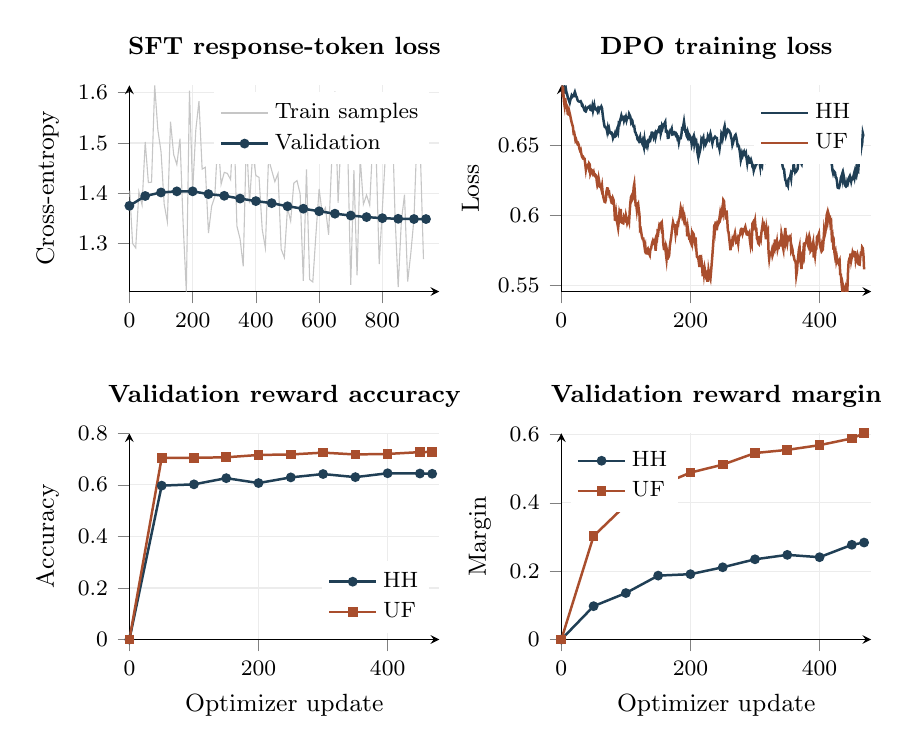
\begin{tikzpicture}
\begin{groupplot}[group style={group size=2 by 2,horizontal sep=1.55cm,vertical sep=1.8cm},reportaxis,width=.455\linewidth,height=4.2cm]
\nextgroupplot[xlabel={},title={SFT response-token loss},ylabel={Cross-entropy},xmin=0,xmax=980,legend pos=north east]
\addplot[gray!45,line width=.4pt] coordinates {(1,1.4050860) (10,1.2998110) (20,1.2909200) (30,1.4029340) (40,1.3765600) (50,1.5018430) (60,1.4211410) (70,1.4219210) (80,1.6146520) (90,1.5259740) (100,1.4827580) (110,1.3780940) (120,1.3431770) (130,1.5422900) (140,1.4770010) (150,1.4570210) (160,1.5086580) (170,1.3379070) (180,1.2038840) (190,1.6043180) (200,1.4048740) (210,1.5258090) (220,1.5833650) (230,1.4479110) (240,1.4515380) (250,1.3206000) (260,1.3737080) (270,1.3928070) (280,1.5129700) (290,1.4177800) (300,1.4413930) (310,1.4392190) (320,1.4269830) (330,1.5534140) (340,1.3343330) (350,1.3088130) (360,1.2544170) (370,1.5114250) (380,1.3797490) (390,1.4808140) (400,1.4352210) (410,1.4313420) (420,1.3279850) (430,1.2908970) (440,1.4689490) (450,1.4454780) (460,1.4227940) (470,1.4392580) (480,1.2883850) (490,1.2718930) (500,1.3705290) (510,1.3444350) (520,1.4199850) (530,1.4250250) (540,1.3985290) (550,1.2251260) (560,1.4471870) (570,1.2279240) (580,1.2230750) (590,1.3189360) (600,1.4084440) (610,1.3590590) (620,1.3708370) (630,1.3169710) (640,1.4670360) (650,1.6026730) (660,1.3807660) (670,1.5221310) (680,1.4809390) (690,1.5021150) (700,1.2173810) (710,1.4457030) (720,1.2360300) (730,1.4706830) (740,1.3778150) (750,1.3963390) (760,1.3760540) (770,1.5097520) (780,1.4862360) (790,1.2588920) (800,1.3686900) (810,1.4802940) (820,1.5858360) (830,1.5751110) (840,1.3564890) (850,1.2127030) (860,1.3438670) (870,1.3969020) (880,1.2236340) (890,1.2802010) (900,1.3497070) (910,1.5227890) (920,1.4833600) (930,1.2684910)};\addlegendentry{Train samples}
\addplot[navy,mark=*,mark size=1.3pt] coordinates {(0,1.3747490) (50,1.3943460) (100,1.4013810) (150,1.4035950) (200,1.4036240) (250,1.3981190) (300,1.3947440) (350,1.3892100) (400,1.3841850) (450,1.3800940) (500,1.3738750) (550,1.3690200) (600,1.3639310) (650,1.3590890) (700,1.3554260) (750,1.3523050) (800,1.3501440) (850,1.3489130) (900,1.3484580) (938,1.3484100)};\addlegendentry{Validation}
\nextgroupplot[xlabel={},title={DPO training loss},ylabel={Loss},xmin=0,xmax=480,legend pos=north east]
\addplot[navy] coordinates {(1,0.6931472) (2,0.6920521) (3,0.6908327) (4,0.6900623) (5,0.6913469) (6,0.6896944) (7,0.6908053) (8,0.6879068) (9,0.6869335) (10,0.6845484) (11,0.6833622) (12,0.6819821) (13,0.6807419) (14,0.6827338) (15,0.6841725) (16,0.6859106) (17,0.6851159) (18,0.6857666) (19,0.6855596) (20,0.6871886) (21,0.6884719) (22,0.6869558) (23,0.6851815) (24,0.6847246) (25,0.6828513) (26,0.6819613) (27,0.6816684) (28,0.6815841) (29,0.6815285) (30,0.6818215) (31,0.6808929) (32,0.6788364) (33,0.6790492) (34,0.6776910) (35,0.6765288) (36,0.6751649) (37,0.6748048) (38,0.6767341) (39,0.6757490) (40,0.6769236) (41,0.6772911) (42,0.6777520) (43,0.6773749) (44,0.6780433) (45,0.6757580) (46,0.6755326) (47,0.6753184) (48,0.6779699) (49,0.6751096) (50,0.6774649) (51,0.6793525) (52,0.6765483) (53,0.6761563) (54,0.6758044) (55,0.6763315) (56,0.6748865) (57,0.6764001) (58,0.6751495) (59,0.6772678) (60,0.6774139) (61,0.6769053) (62,0.6780194) (63,0.6768993) (64,0.6726176) (65,0.6692210) (66,0.6663334) (67,0.6636888) (68,0.6634863) (69,0.6625620) (70,0.6624374) (71,0.6600545) (72,0.6628097) (73,0.6604569) (74,0.6620469) (75,0.6596908) (76,0.6591258) (77,0.6595521) (78,0.6593348) (79,0.6579990) (80,0.6555146) (81,0.6568386) (82,0.6567530) (83,0.6584290) (84,0.6568014) (85,0.6572221) (86,0.6614547) (87,0.6627694) (88,0.6607609) (89,0.6660186) (90,0.6655568) (91,0.6681433) (92,0.6695587) (93,0.6715057) (94,0.6697697) (95,0.6706765) (96,0.6705817) (97,0.6680709) (98,0.6698015) (99,0.6690324) (100,0.6705222) (101,0.6681516) (102,0.6699115) (103,0.6699867) (104,0.6699345) (105,0.6726958) (106,0.6717425) (107,0.6705394) (108,0.6673903) (109,0.6686601) (110,0.6679989) (111,0.6647822) (112,0.6636927) (113,0.6638924) (114,0.6600907) (115,0.6593910) (116,0.6578326) (117,0.6573247) (118,0.6545730) (119,0.6541377) (120,0.6533525) (121,0.6550895) (122,0.6564521) (123,0.6530803) (124,0.6532112) (125,0.6520547) (126,0.6536482) (127,0.6511345) (128,0.6489806) (129,0.6540310) (130,0.6508317) (131,0.6498528) (132,0.6525720) (133,0.6531374) (134,0.6506478) (135,0.6533258) (136,0.6531428) (137,0.6551809) (138,0.6544494) (139,0.6563726) (140,0.6594155) (141,0.6593985) (142,0.6585210) (143,0.6562471) (144,0.6578487) (145,0.6588905) (146,0.6557866) (147,0.6576908) (148,0.6599662) (149,0.6597826) (150,0.6608913) (151,0.6604464) (152,0.6635933) (153,0.6637918) (154,0.6585946) (155,0.6604283) (156,0.6642470) (157,0.6631010) (158,0.6650626) (159,0.6649871) (160,0.6661709) (161,0.6671112) (162,0.6604410) (163,0.6607149) (164,0.6605966) (165,0.6556398) (166,0.6556836) (167,0.6579023) (168,0.6594352) (169,0.6609774) (170,0.6606274) (171,0.6619810) (172,0.6579883) (173,0.6581147) (174,0.6597631) (175,0.6597970) (176,0.6590326) (177,0.6578141) (178,0.6586836) (179,0.6580172) (180,0.6550749) (181,0.6555849) (182,0.6524645) (183,0.6550159) (184,0.6553681) (185,0.6553893) (186,0.6579384) (187,0.6622773) (188,0.6620571) (189,0.6645123) (190,0.6673339) (191,0.6638846) (192,0.6605583) (193,0.6607695) (194,0.6571927) (195,0.6562327) (196,0.6594791) (197,0.6577019) (198,0.6557989) (199,0.6570644) (200,0.6561067) (201,0.6543853) (202,0.6508442) (203,0.6526910) (204,0.6558987) (205,0.6569917) (206,0.6514442) (207,0.6541461) (208,0.6522850) (209,0.6531056) (210,0.6492097) (211,0.6446503) (212,0.6422455) (213,0.6468563) (214,0.6448590) (215,0.6468280) (216,0.6491342) (217,0.6544620) (218,0.6534454) (219,0.6546962) (220,0.6558888) (221,0.6515391) (222,0.6536232) (223,0.6538740) (224,0.6514111) (225,0.6525061) (226,0.6535650) (227,0.6567637) (228,0.6555877) (229,0.6545965) (230,0.6566720) (231,0.6586041) (232,0.6567043) (233,0.6539018) (234,0.6516437) (235,0.6538975) (236,0.6547277) (237,0.6557165) (238,0.6563787) (239,0.6557296) (240,0.6557121) (241,0.6554978) (242,0.6498958) (243,0.6500855) (244,0.6496067) (245,0.6475201) (246,0.6512581) (247,0.6526866) (248,0.6585964) (249,0.6575856) (250,0.6552952) (251,0.6578239) (252,0.6622261) (253,0.6640303) (254,0.6607309) (255,0.6573078) (256,0.6588960) (257,0.6600214) (258,0.6615490) (259,0.6611930) (260,0.6606740) (261,0.6592764) (262,0.6587919) (263,0.6559035) (264,0.6544808) (265,0.6505733) (266,0.6519411) (267,0.6540448) (268,0.6560787) (269,0.6572576) (270,0.6578554) (271,0.6559485) (272,0.6534301) (273,0.6500975) (274,0.6504267) (275,0.6496027) (276,0.6470650) (277,0.6440237) (278,0.6396928) (279,0.6417182) (280,0.6446151) (281,0.6431567) (282,0.6448464) (283,0.6458084) (284,0.6441546) (285,0.6432554) (286,0.6444460) (287,0.6407547) (288,0.6374903) (289,0.6406633) (290,0.6415978) (291,0.6405718) (292,0.6379109) (293,0.6378827) (294,0.6395359) (295,0.6378780) (296,0.6353273) (297,0.6356221) (298,0.6321498) (299,0.6337838) (300,0.6344178) (301,0.6359918) (302,0.6365185) (303,0.6376601) (304,0.6382874) (305,0.6384631) (306,0.6387063) (307,0.6380066) (308,0.6351368) (309,0.6410672) (310,0.6374732) (311,0.6360992) (312,0.6419056) (313,0.6482560) (314,0.6448015) (315,0.6426843) (316,0.6490374) (317,0.6557106) (318,0.6563376) (319,0.6550620) (320,0.6567620) (321,0.6615591) (322,0.6638345) (323,0.6663665) (324,0.6658960) (325,0.6655916) (326,0.6637833) (327,0.6586300) (328,0.6590170) (329,0.6557183) (330,0.6531882) (331,0.6538770) (332,0.6477998) (333,0.6498579) (334,0.6480796) (335,0.6485828) (336,0.6520355) (337,0.6506785) (338,0.6471205) (339,0.6481993) (340,0.6491712) (341,0.6439623) (342,0.6374351) (343,0.6348700) (344,0.6333950) (345,0.6330623) (346,0.6283651) (347,0.6253900) (348,0.6247483) (349,0.6220214) (350,0.6224207) (351,0.6213042) (352,0.6261978) (353,0.6268023) (354,0.6269255) (355,0.6290164) (356,0.6265553) (357,0.6316185) (358,0.6318448) (359,0.6326186) (360,0.6380239) (361,0.6331966) (362,0.6312741) (363,0.6323884) (364,0.6317501) (365,0.6324112) (366,0.6334195) (367,0.6388319) (368,0.6392255) (369,0.6386237) (370,0.6401224) (371,0.6387283) (372,0.6431463) (373,0.6403039) (374,0.6443857) (375,0.6472469) (376,0.6471487) (377,0.6482600) (378,0.6495793) (379,0.6536763) (380,0.6523512) (381,0.6550282) (382,0.6512434) (383,0.6513493) (384,0.6495094) (385,0.6462349) (386,0.6528984) (387,0.6546722) (388,0.6546715) (389,0.6554521) (390,0.6601138) (391,0.6555679) (392,0.6555996) (393,0.6557868) (394,0.6582209) (395,0.6560684) (396,0.6608595) (397,0.6569519) (398,0.6611719) (399,0.6610885) (400,0.6608938) (401,0.6642304) (402,0.6622419) (403,0.6632973) (404,0.6610408) (405,0.6586653) (406,0.6568832) (407,0.6590565) (408,0.6544813) (409,0.6530441) (410,0.6524474) (411,0.6507800) (412,0.6458033) (413,0.6465930) (414,0.6477789) (415,0.6426631) (416,0.6438536) (417,0.6378346) (418,0.6375915) (419,0.6367785) (420,0.6323402) (421,0.6302894) (422,0.6319026) (423,0.6313220) (424,0.6306826) (425,0.6273464) (426,0.6270455) (427,0.6243509) (428,0.6201215) (429,0.6197529) (430,0.6197137) (431,0.6213827) (432,0.6232789) (433,0.6271132) (434,0.6282264) (435,0.6297460) (436,0.6261159) (437,0.6294021) (438,0.6270866) (439,0.6241487) (440,0.6213220) (441,0.6207876) (442,0.6212954) (443,0.6243613) (444,0.6231933) (445,0.6249723) (446,0.6274332) (447,0.6283995) (448,0.6267092) (449,0.6244676) (450,0.6267070) (451,0.6263840) (452,0.6273791) (453,0.6292698) (454,0.6272842) (455,0.6311610) (456,0.6296173) (457,0.6337800) (458,0.6309544) (459,0.6337301) (460,0.6327782) (461,0.6390682) (462,0.6419456) (463,0.6434047) (464,0.6465139) (465,0.6495487) (466,0.6512432) (467,0.6589968) (468,0.6570805) (469,0.6571629)};\addlegendentry{HH}
\addplot[rust] coordinates {(1,0.6931472) (2,0.6880013) (3,0.6890365) (4,0.6818896) (5,0.6788157) (6,0.6841409) (7,0.6797924) (8,0.6793563) (9,0.6764758) (10,0.6727012) (11,0.6724512) (12,0.6750722) (13,0.6731567) (14,0.6711195) (15,0.6687600) (16,0.6666673) (17,0.6650465) (18,0.6634428) (19,0.6589600) (20,0.6592782) (21,0.6567702) (22,0.6536131) (23,0.6543058) (24,0.6523297) (25,0.6513030) (26,0.6517953) (27,0.6507770) (28,0.6478926) (29,0.6465325) (30,0.6471890) (31,0.6442472) (32,0.6421765) (33,0.6413947) (34,0.6418548) (35,0.6406882) (36,0.6406445) (37,0.6369898) (38,0.6330315) (39,0.6360741) (40,0.6358494) (41,0.6363082) (42,0.6345173) (43,0.6373009) (44,0.6366014) (45,0.6297804) (46,0.6309447) (47,0.6325641) (48,0.6321373) (49,0.6303016) (50,0.6312985) (51,0.6286975) (52,0.6282435) (53,0.6291738) (54,0.6286961) (55,0.6240868) (56,0.6210885) (57,0.6220324) (58,0.6260931) (59,0.6233431) (60,0.6209969) (61,0.6212206) (62,0.6191098) (63,0.6215189) (64,0.6166021) (65,0.6134033) (66,0.6115107) (67,0.6098082) (68,0.6096286) (69,0.6114096) (70,0.6175256) (71,0.6194570) (72,0.6193867) (73,0.6161247) (74,0.6165509) (75,0.6132961) (76,0.6132665) (77,0.6106806) (78,0.6090929) (79,0.6088333) (80,0.6122561) (81,0.6110707) (82,0.6061121) (83,0.5970826) (84,0.5968958) (85,0.6009309) (86,0.5964493) (87,0.5938684) (88,0.5911567) (89,0.5956603) (90,0.6021602) (91,0.6004890) (92,0.6047352) (93,0.5952583) (94,0.5949594) (95,0.5946855) (96,0.5944737) (97,0.5985281) (98,0.5971240) (99,0.5965210) (100,0.6000817) (101,0.5977016) (102,0.5947343) (103,0.5962081) (104,0.5976139) (105,0.5957184) (106,0.6036213) (107,0.6095091) (108,0.6134680) (109,0.6143808) (110,0.6114703) (111,0.6123682) (112,0.6200810) (113,0.6225403) (114,0.6154289) (115,0.6080242) (116,0.6082498) (117,0.6038965) (118,0.6074827) (119,0.6084255) (120,0.6041516) (121,0.6009189) (122,0.5897691) (123,0.5903541) (124,0.5873963) (125,0.5845261) (126,0.5832756) (127,0.5834168) (128,0.5805127) (129,0.5772935) (130,0.5787319) (131,0.5731262) (132,0.5730150) (133,0.5755255) (134,0.5762292) (135,0.5743041) (136,0.5726696) (137,0.5716589) (138,0.5759623) (139,0.5764425) (140,0.5789563) (141,0.5809762) (142,0.5823305) (143,0.5814057) (144,0.5801119) (145,0.5817662) (146,0.5748375) (147,0.5802380) (148,0.5814348) (149,0.5879267) (150,0.5871610) (151,0.5907384) (152,0.5936170) (153,0.5930042) (154,0.5939489) (155,0.5911849) (156,0.5930102) (157,0.5881541) (158,0.5793768) (159,0.5760552) (160,0.5759877) (161,0.5777929) (162,0.5726645) (163,0.5687524) (164,0.5740753) (165,0.5715968) (166,0.5703662) (167,0.5713428) (168,0.5779896) (169,0.5812527) (170,0.5841213) (171,0.5880729) (172,0.5921400) (173,0.5951847) (174,0.5933987) (175,0.5932560) (176,0.5918933) (177,0.5870022) (178,0.5903791) (179,0.5891074) (180,0.5940753) (181,0.5935362) (182,0.5971385) (183,0.5982028) (184,0.6015095) (185,0.6055489) (186,0.6036914) (187,0.6007033) (188,0.6027334) (189,0.5978211) (190,0.5960610) (191,0.5984689) (192,0.5954496) (193,0.5941438) (194,0.5943385) (195,0.5852603) (196,0.5906159) (197,0.5871572) (198,0.5839377) (199,0.5842485) (200,0.5813961) (201,0.5802628) (202,0.5851658) (203,0.5820088) (204,0.5874421) (205,0.5867299) (206,0.5835901) (207,0.5807766) (208,0.5843482) (209,0.5765631) (210,0.5706227) (211,0.5700283) (212,0.5701013) (213,0.5665099) (214,0.5631763) (215,0.5718939) (216,0.5670744) (217,0.5684031) (218,0.5643081) (219,0.5565366) (220,0.5634960) (221,0.5584645) (222,0.5624490) (223,0.5599553) (224,0.5571124) (225,0.5581403) (226,0.5534519) (227,0.5534649) (228,0.5607606) (229,0.5577505) (230,0.5564746) (231,0.5548269) (232,0.5601528) (233,0.5658984) (234,0.5718087) (235,0.5780294) (236,0.5848482) (237,0.5937055) (238,0.5901590) (239,0.5957057) (240,0.5902841) (241,0.5902675) (242,0.5945559) (243,0.5938181) (244,0.5949207) (245,0.5983276) (246,0.6015960) (247,0.5989033) (248,0.6007854) (249,0.6040347) (250,0.6021373) (251,0.6110917) (252,0.6103457) (253,0.6036646) (254,0.6013782) (255,0.5972820) (256,0.6035845) (257,0.5969168) (258,0.5892976) (259,0.5881634) (260,0.5839907) (261,0.5798666) (262,0.5751360) (263,0.5805592) (264,0.5797243) (265,0.5827355) (266,0.5812490) (267,0.5840199) (268,0.5854236) (269,0.5874140) (270,0.5840828) (271,0.5807473) (272,0.5811132) (273,0.5829059) (274,0.5799368) (275,0.5846332) (276,0.5856830) (277,0.5862938) (278,0.5900300) (279,0.5905358) (280,0.5903799) (281,0.5872948) (282,0.5888425) (283,0.5888555) (284,0.5907568) (285,0.5920006) (286,0.5898505) (287,0.5865927) (288,0.5864139) (289,0.5875314) (290,0.5868626) (291,0.5877860) (292,0.5826624) (293,0.5791946) (294,0.5827465) (295,0.5805201) (296,0.5942994) (297,0.5951328) (298,0.5923663) (299,0.5938425) (300,0.5961547) (301,0.5903341) (302,0.5904288) (303,0.5836127) (304,0.5827773) (305,0.5802060) (306,0.5796438) (307,0.5846187) (308,0.5846863) (309,0.5830620) (310,0.5879208) (311,0.5910092) (312,0.5943045) (313,0.5918405) (314,0.5930287) (315,0.5900184) (316,0.5872681) (317,0.5830192) (318,0.5905006) (319,0.5875417) (320,0.5888268) (321,0.5739883) (322,0.5691796) (323,0.5726773) (324,0.5718648) (325,0.5723207) (326,0.5745448) (327,0.5712187) (328,0.5728119) (329,0.5772873) (330,0.5762185) (331,0.5829249) (332,0.5771214) (333,0.5783650) (334,0.5811985) (335,0.5763111) (336,0.5785017) (337,0.5778842) (338,0.5806413) (339,0.5816119) (340,0.5778661) (341,0.5868218) (342,0.5843129) (343,0.5780227) (344,0.5757399) (345,0.5838466) (346,0.5866655) (347,0.5911084) (348,0.5812032) (349,0.5831271) (350,0.5803559) (351,0.5839881) (352,0.5832900) (353,0.5844720) (354,0.5834670) (355,0.5844103) (356,0.5760469) (357,0.5777396) (358,0.5759661) (359,0.5716056) (360,0.5711856) (361,0.5684531) (362,0.5675518) (363,0.5668004) (364,0.5572576) (365,0.5602240) (366,0.5666538) (367,0.5711072) (368,0.5756258) (369,0.5777983) (370,0.5674221) (371,0.5660213) (372,0.5617240) (373,0.5703100) (374,0.5690388) (375,0.5750159) (376,0.5726109) (377,0.5801294) (378,0.5802829) (379,0.5806619) (380,0.5833644) (381,0.5805116) (382,0.5790239) (383,0.5835873) (384,0.5855409) (385,0.5834572) (386,0.5745574) (387,0.5752669) (388,0.5751279) (389,0.5785216) (390,0.5807040) (391,0.5700388) (392,0.5749647) (393,0.5714536) (394,0.5763016) (395,0.5764201) (396,0.5845085) (397,0.5854237) (398,0.5858499) (399,0.5871353) (400,0.5802305) (401,0.5779581) (402,0.5762450) (403,0.5784249) (404,0.5749982) (405,0.5756742) (406,0.5810064) (407,0.5890641) (408,0.5859731) (409,0.5878906) (410,0.5928604) (411,0.6003943) (412,0.6020573) (413,0.5974777) (414,0.6010043) (415,0.5992770) (416,0.5992605) (417,0.5934335) (418,0.5946434) (419,0.5847511) (420,0.5860059) (421,0.5795310) (422,0.5808385) (423,0.5737608) (424,0.5706812) (425,0.5727818) (426,0.5675855) (427,0.5697027) (428,0.5668185) (429,0.5659044) (430,0.5671916) (431,0.5681607) (432,0.5581161) (433,0.5578600) (434,0.5517813) (435,0.5474642) (436,0.5503847) (437,0.5478365) (438,0.5467555) (439,0.5473198) (440,0.5488172) (441,0.5460195) (442,0.5461829) (443,0.5456183) (444,0.5586974) (445,0.5669374) (446,0.5688461) (447,0.5686474) (448,0.5729174) (449,0.5678522) (450,0.5703669) (451,0.5732266) (452,0.5713140) (453,0.5719620) (454,0.5739155) (455,0.5737515) (456,0.5680257) (457,0.5702975) (458,0.5687430) (459,0.5716146) (460,0.5697973) (461,0.5650587) (462,0.5648783) (463,0.5697931) (464,0.5731493) (465,0.5729060) (466,0.5773160) (467,0.5765675) (468,0.5718710) (469,0.5615403)};\addlegendentry{UF}
\nextgroupplot[title={Validation reward accuracy},ylabel={Accuracy},ymin=0,ymax=.8,xmin=0,xmax=480,legend pos=south east]
\addplot[navy,mark=*,mark size=1.3pt] coordinates {(0,0.0000000) (50,0.5970000) (100,0.6020000) (150,0.6260000) (200,0.6070000) (250,0.6290000) (300,0.6420000) (350,0.6300000) (400,0.6450000) (450,0.6440000) (469,0.6430000)};\addlegendentry{HH}
\addplot[rust,mark=square*,mark size=1.3pt] coordinates {(0,0.0000000) (50,0.7050000) (100,0.7050000) (150,0.7070000) (200,0.7160000) (250,0.7180000) (300,0.7250000) (350,0.7180000) (400,0.7200000) (450,0.7270000) (469,0.7280000)};\addlegendentry{UF}
\nextgroupplot[title={Validation reward margin},ylabel={Margin},xmin=0,xmax=480,legend pos=north west]
\addplot[navy,mark=*,mark size=1.3pt] coordinates {(0,0.0000000) (50,0.0975588) (100,0.1359562) (150,0.1869639) (200,0.1911604) (250,0.2113482) (300,0.2347276) (350,0.2477031) (400,0.2408797) (450,0.2771887) (469,0.2837627)};\addlegendentry{HH}
\addplot[rust,mark=square*,mark size=1.3pt] coordinates {(0,0.0000000) (50,0.3028129) (100,0.3939285) (150,0.4487368) (200,0.4884938) (250,0.5117742) (300,0.5457390) (350,0.5550223) (400,0.5687939) (450,0.5884993) (469,0.6034576)};\addlegendentry{UF}
\end{groupplot}
\end{tikzpicture}
\caption{SFT train samples and validation points are unsmoothed. DPO train loss uses a trailing 25-update mean. The identical initial policy and reference give 0 strict reward accuracy and 0 margin.}
\label{fig:training}
\end{figure}



Both DPO runs completed 469 updates over 15,000 pairs, with no skipped updates and unchanged frozen references. UF developed stronger preference separation than HH: 72.8\% versus 64.5\% selected validation accuracy, and 0.6035 versus 0.2409 reward margin.
\begin{table}[H]
\centering\small
\begin{tabular}{@{}lrrrrr@{}}\toprule
Track & Selected / final & Val. loss, selected / final & Selected accuracy & Margin & Final accuracy\\\midrule
HH & 400 / 469 & 0.630991 / 0.622583 & 64.5\% & 0.240880 & 64.3\%\\
UF & 469 / 469 & 0.553575 / 0.553575 & 72.8\% & 0.603458 & 72.8\%\\\bottomrule
\end{tabular}
\caption{General DPO checkpoints selected by validation reward accuracy.}
\end{table}
HH's loss continued to fall after update 400, but its preference accuracy ended 0.2 percentage points lower. I therefore evaluated update 400. UF's highest accuracy occurred at its final update.

\Needspace{5\baselineskip}
Persona reached \textbf{100\% accuracy on 22 validation pairs at update 5}, then tied it at updates 10 and 13. The first maximum selected update 5. Validation loss fell from 0.693147 to 0.690129 at selection and 0.685189 at the end; margin rose to 0.006046 and 0.015986. The frozen base weights stayed unchanged.

\begin{figure}[!ht]
\centering
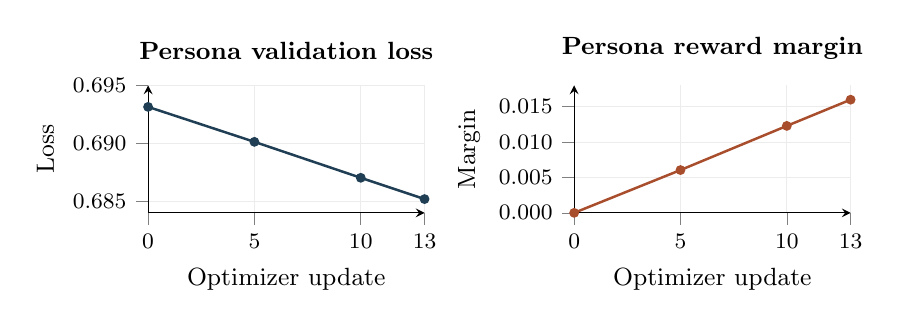
\begin{tikzpicture}
\begin{groupplot}[group style={group size=2 by 1,horizontal sep=1.9cm},reportaxis,width=.42\linewidth,height=3.2cm,xmin=0,xmax=13,xtick={0,5,10,13}]
\nextgroupplot[title={Persona validation loss},ylabel={Loss},ymin=.684,ymax=.695,ytick={.685,.690,.695},yticklabel style={/pgf/number format/fixed,/pgf/number format/precision=3,/pgf/number format/fixed zerofill}]
\addplot[navy,mark=*,mark size=1.3pt] coordinates {(0,.693147)(5,.690129)(10,.687027)(13,.685189)};
\nextgroupplot[title={Persona reward margin},ylabel={Margin},ymin=0,ymax=.018,ytick={0,.005,.010,.015},yticklabel style={/pgf/number format/fixed,/pgf/number format/precision=3,/pgf/number format/fixed zerofill}]
\addplot[rust,mark=*,mark size=1.3pt] coordinates {(0,0)(5,.006046)(10,.012282)(13,.015986)};
\end{groupplot}
\end{tikzpicture}
\caption{Persona validation loss and margin, unsmoothed. Best checkpoint: update 5, the first to reach 100\% preference accuracy.}
\label{fig:persona}
\end{figure}



\section{DPO-versus-SFT results}
I generated 300 answers per bank: base on Alpaca, plus SFT, HH DPO, and UF DPO on both Alpaca and HH, giving 2,100 saved answers with no blanks. Four separate files compare DPO against SFT; A/B positions are randomized with seed 42 and model identities are hidden from the judge.

The judge was \model{google/gemini-3.6-flash} through Kaggle Benchmarks SDK 0.6.1. It compared correctness, helpfulness, instruction following, concision, formatting, hallucinations, and safety. Requests contained five pairs, with at least five seconds between attempts and up to three attempts per batch. Valid ID-matched judgments were saved after each batch; malformed or missing decisions were retried, and unresolved failures were logged. All 1,200 pairs were judged: \textbf{250 attempts, 10 retries, zero unknowns or unresolved failures}. HH/Alpaca needed one retry and UF/Alpaca nine.

\begin{table}[H]
\centering\small
\begin{tabularx}{\linewidth}{@{}lrrrYYY@{}}\toprule
DPO / set & Wins & Ties & Losses & Tie-adjusted & Decisive & 95\% interval\\\midrule
HH / Alpaca & 101 & 98 & 101 & 50.0\% & 50.0\% & 45.3--54.5\%\\
HH / HH & 115 & 47 & 138 & 46.2\% & 45.5\% & 38.9--53.2\%\\
UF / Alpaca & 91 & 63 & 146 & 40.8\% & 38.4\% & 36.2--45.7\%\\
UF / HH & 103 & 24 & 173 & 38.3\% & 37.3\% & 31.0--45.7\%\\\bottomrule
\end{tabularx}
\caption{DPO against SFT; 300 valid judgments per row. Tie-adjusted rate is $(W+T/2)/300$; decisive rate is $W/(W+L)$. Intervals use 2,000 seed-42 bootstrap resamples, clustered by instruction for HH.}
\end{table}

\textbf{HH tied SFT on Alpaca}: 101 wins and 101 losses. On HH it lost 138 pairs and won 115, placing its tie-adjusted score 3.8 points below parity. Both intervals include 50\%. \textbf{UF lost to SFT on both sets}, finishing 9.2 points below parity on Alpaca and 11.7 below on HH; both intervals are below 50\%. The run with the stronger preference metrics generated the weaker judged answers.

\subsection*{Persona result}
\begin{table}[H]
\centering\small
\begin{tabular}{@{}lrrrr@{}}\toprule
Adapter & Val. loss & Val. accuracy & Margin & Changed answers\\\midrule
Best, update 5 & 0.690129 & 100\% & 0.006046 & 2/40\\
Final, update 13 & 0.685189 & 100\% & 0.015986 & 6/40\\\bottomrule
\end{tabular}
\caption{Persona compared with the unmodified SmolLM2 baseline on the same 40 prompts and decoder.}
\end{table}
Neither checkpoint developed a distinct Ramsay voice. Every coding answer stayed unchanged. A changed salmon answer added closing advice but retained unsafe doneness guidance; cake-rescue advice remained unsound, and a changed correlation/causation explanation remained confused. Allergy-prank and password-theft responses remained harmful. Baseline, best, and final each reached the token cap on 22/40 prompts. This was a matched manual comparison, with no external persona judging.

\section{Interpretation and error analysis}
The following examples use the final decoder on the 40-prompt development bank. They show improvement, regression, and unchanged behavior alongside the larger judged comparisons.
\begin{table}[H]
\centering\small
\begin{tabularx}{\linewidth}{@{}p{.25\linewidth}YYY@{}}\toprule
Prompt / expected result & SFT & HH DPO & UF DPO\\\midrule
Beads: $18+12-6+3=27$ & 27, but calls the total a blue-bead count & 9; loses bead counts and colors & 27, with consistent color accounting\\
Bat and ball: 110 cents total; bat costs 100 cents more; ball costs 5 & 5, with correct algebra & Writes $2x+100=110$, then answers 50 & 5, with correct algebra\\
Maya books Friday; Omar sends invitations Monday & Extracts both actions & Extracts both actions & Extracts both actions\\
Integer counts: \texttt{\{2:3, -3:2\}} & Correct function; wrong example comment & Correct function; wrong example comment & Correct function; wrong example comment\\
Planet-name lengths: three executable cases & 3/3 pass & 3/3 pass & Counts occurrences; 1/3 pass\\\bottomrule
\end{tabularx}
\caption{Matched development outputs. Full answers: \texttt{evaluation/*-development.json}.}
\end{table}

UF improved the bead explanation while retaining the correct total. HH regressed on both arithmetic tasks: even a correct equation did not lead to the correct bat-and-ball answer. Extraction stayed the same, and DPO did not fix the incorrect comment attached to the counting function. Persona likewise retained its coding errors: first-unique-character failed \texttt{aab}, \texttt{abc}, and \texttt{aabb}; binary search passed four edge cases. A 90-minute plan still totaled 135 minutes, and a library summary invented closing times.

\textbf{UF's failures extended beyond isolated examples.} Its answers reached the 256-token cap on 138/300 Alpaca prompts and 163/300 HH prompts, compared with 56 and 52 for SFT, and 41 and 34 for HH DPO. Final banks contained repeated ``please'' in a landlord-message rewrite, repeated hashtags, and an HH DPO emoji loop. Raising the repetition penalty fixed a development loop but did not remove repetition from the evaluation banks.

\textbf{Preference data and response coverage help explain the mismatch.} Pair reviews found factual errors and mismatched refusals among chosen responses in both datasets; source checks found no converter label swap. UF truncated chosen responses in \textbf{3,987/15,000 pairs}, compared with \textbf{28/15,000 for HH}. Sampled chosen/rejected length ratios averaged 1.96 and 1.60. The response-summed objective therefore trained on labels and response spans that did not consistently represent a better complete answer. These observations support data mismatch as an explanation; the runs did not vary filtering or context length to measure its individual effect.

The general runs held $\beta=0.1$ and training length at one epoch, so they provide a direct comparison of the two preference sources from the same SFT origin. UF's larger reward margin accompanied worse generation; HH's smaller margin accompanied parity on Alpaca and a lower score on HH. Lower DPO loss and higher preference accuracy did not predict the ordering of answer quality. Persona showed the other failure: margins of only 0.0060--0.0160 changed pair rankings while leaving most greedy answers identical. Its small adapter and short, low-LR run achieved preference separation without the intended style transfer.

\section{Limitations and reproducibility}
Training used one seed and general evaluation one model judge. Bootstrap intervals cover prompt-sampling variation, not judge bias or training-seed variance. Exact prompt exclusions do not detect semantic overlap. HH repeats instructions; the persona comparison contains 22 validation pairs and 40 manually selected evaluation prompts and was unblinded. There was no controlled sweep of $\beta$, context length, or training duration.

\begin{table}[H]
\centering\footnotesize
\begin{tabularx}{\linewidth}{@{}lY@{}}\toprule
Reproduce & Repository files\\\midrule
Data and settings & \pathcode{data/general/}, \pathcode{configs/}, \pathcode{evidence/data_summary.json}\\
Training curves and checkpoints & \pathcode{evidence/sft-launch_status.json}, \pathcode{evidence/sft-completed-run-logs.txt}, \pathcode{evidence/dpo/}, \pathcode{evidence/persona-best/}, \pathcode{evidence/persona-final/}\\
Answers and judge results & \pathcode{evaluation/matched/}, \pathcode{evaluation/judged/}, \pathcode{evaluation/summary.json}, \pathcode{scripts/summarize_saved_evaluation.py}\\
Kaggle workflows & \pathcode{notebooks/01_Qwen_Training.ipynb}, \pathcode{02_Matched_Generation.ipynb}, \pathcode{03_Saved_Pair_Judging.ipynb}, \pathcode{04_Persona_LoRA.ipynb} (all under \texttt{notebooks/})\\\bottomrule
\end{tabularx}
\end{table}
Qwen runs used PyTorch 2.11.0+cu128 and Transformers 4.57.6; persona used Transformers 4.51.3, TRL 0.19.1, and PEFT 0.15.2.

Large weights are saved in the original private Kaggle outputs; checkpoint paths and SHA256 values are included in the run records. Saved versions: SFT 356840240, DPO 357186707, generation 357326672, judging 357378242, persona best 357420502 and final 357446665. The saved answers and judgments reproduce every result table without downloading weights.

SFT remains the stronger model against UF on both evaluation sets. HH did not improve over SFT, and persona preference accuracy did not translate into a useful style change. The result is that these preference-training runs improved their own validation objectives without improving the assistant behavior they were meant to target.

\begin{thebibliography}{3}\small
\setlength{\itemsep}{1pt}\setlength{\parskip}{0pt}
\bibitem{dpo} R. Rafailov et al. \emph{Direct Preference Optimization: Your Language Model is Secretly a Reward Model}. NeurIPS, 2023. \href{https://arxiv.org/abs/2305.18290}{arXiv:2305.18290}.
\bibitem{trl} Hugging Face. \emph{TRL DPOTrainer}, version 0.19.1. \url{https://huggingface.co/docs/trl/v0.19.1/en/dpo_trainer}.
\bibitem{peft} Hugging Face. \emph{PEFT LoRA configuration reference}. \url{https://huggingface.co/docs/peft/package_reference/lora}. Executed version: 0.15.2.
\end{thebibliography}
\end{document}
